\section{Regression accuracy}
This section includes an examination of the accuracy of the regressors. This will be examined through superimposition of the regressor outputs on the estimated data, and through RMSE plots. To evaluate how the regressors perform with new data, a test with new data of 50 $\%$ of the MVC of all movements in all limb positions will be fed the regressor and the above examination of accuracy will be performed. 

The plot in \figref{fig:SuperPositionTestDataLogVar} depicts the actual data superimposed on the estimated data from the regressors trained with the LogVar features. 

\begin{figure}[H]
	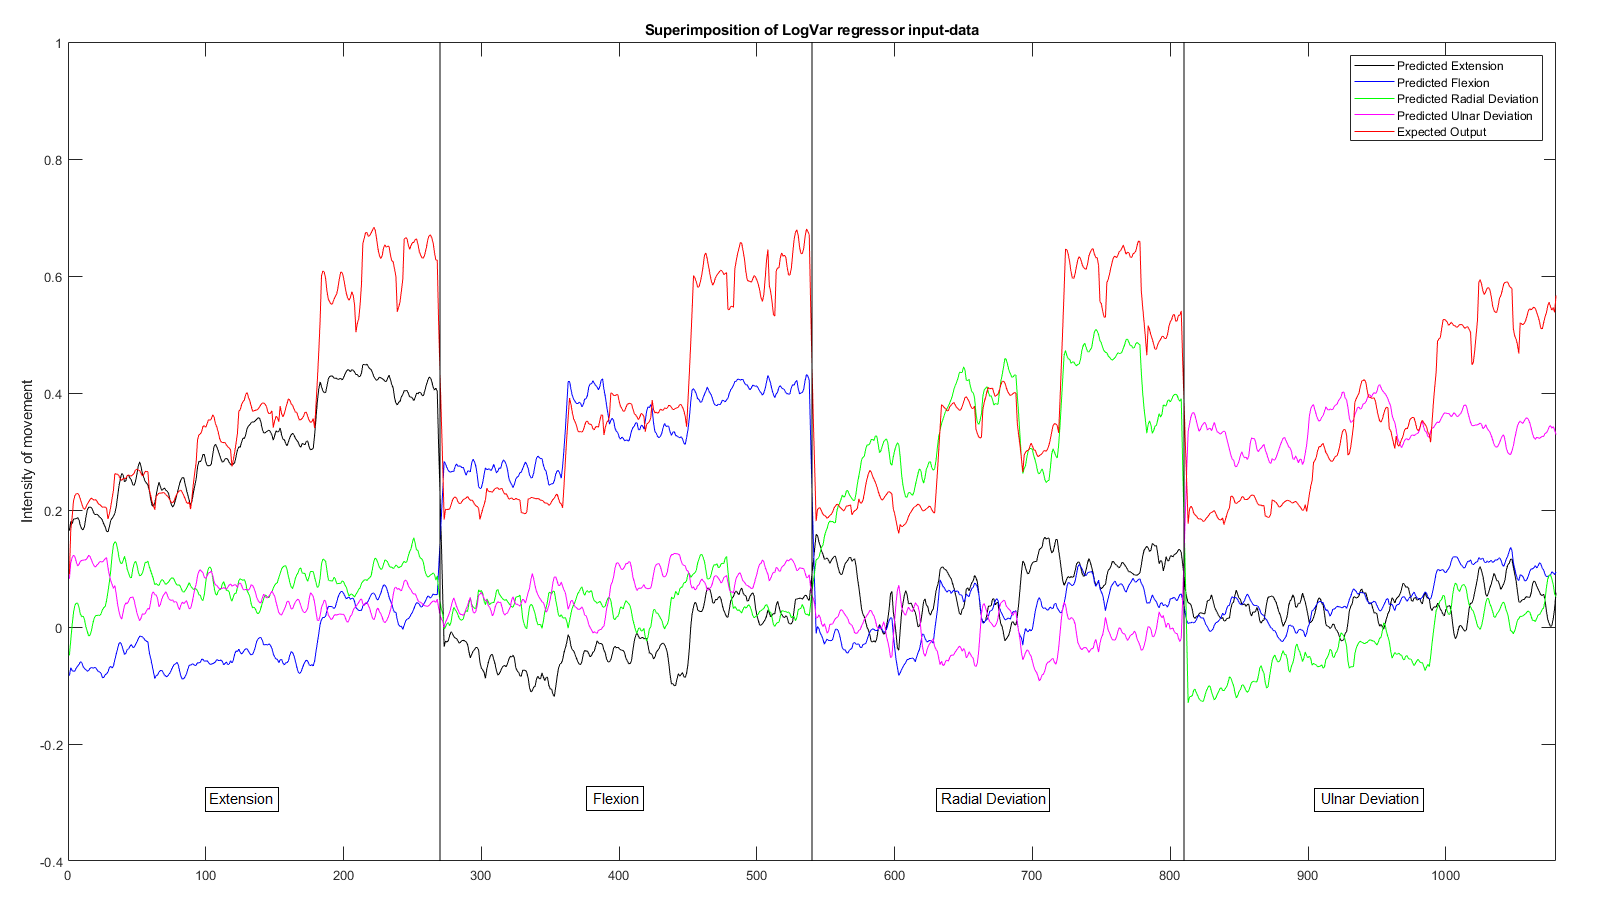
\includegraphics[width=1\textwidth]{figures/results/SuperPositionTestDataLogVar}  %<--but is not needed.
	\caption{Plot of the actual data, red plot, superimposed on the output of the regressors trained with the LogVar features. The plot is divided into four segments, where each segment shows a different movement performed. Each segment has the same sample size.}
	\label{fig:SuperPositionTestDataLogVar}  %<--give the figure a label, so you can reference!
\end{figure}

The plot in \figref{fig:SuperPositionTestDataMAV} depicts the actual data superimposed on the estimated data from the regressors trained with the MAV features. 

\begin{figure}[H]
	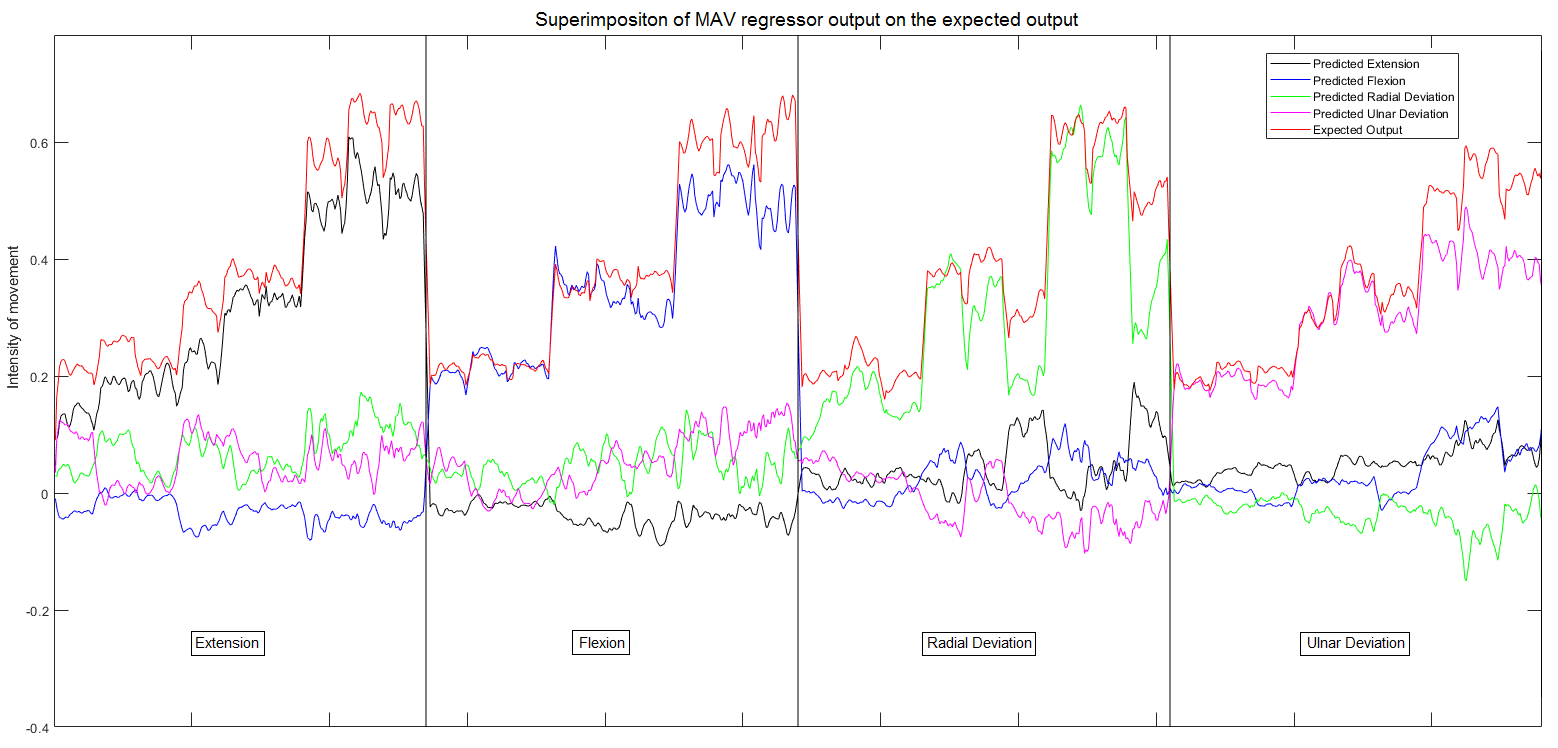
\includegraphics[width=1\textwidth]{figures/results/SuperPositionTestDataMAV}  %<--but is not needed.
	\caption{Plot of the actual data, red plot, superimposed on the output of the regressors trained with the MAV features. The plot is divided into four segments, where each segment shows a different movement performed. Each segment has the same sample size.}
	\label{fig:SuperPositionTestDataMAV}  %<--give the figure a label, so you can reference!
\end{figure}


A qualitative examination of the plots shows that each regressor reacts on the movement it is fitted for, and remains inactive when another movement is performed. This accounts for both features. Both regressors has a lower accuracy in the high intensities, especially for the regressors trained with logarithmic variance features. 
%regression on MAV features yields a more accurate output than regression on the logarithmic variance feature, whereas both estimates yield inaccurate fitting in the high intensities. However, both estimates yield inaccurate fitting in the high intensities compared to the lower intensities, especially in the ulnar deviation movement.
  


Calculating the RMSE of the regressors for the MAV and LogVar features of the training data across all subjects, yields the results depicted in \figref{fig:gimmeThemRMSEBars}. 

\begin{figure}[H]
	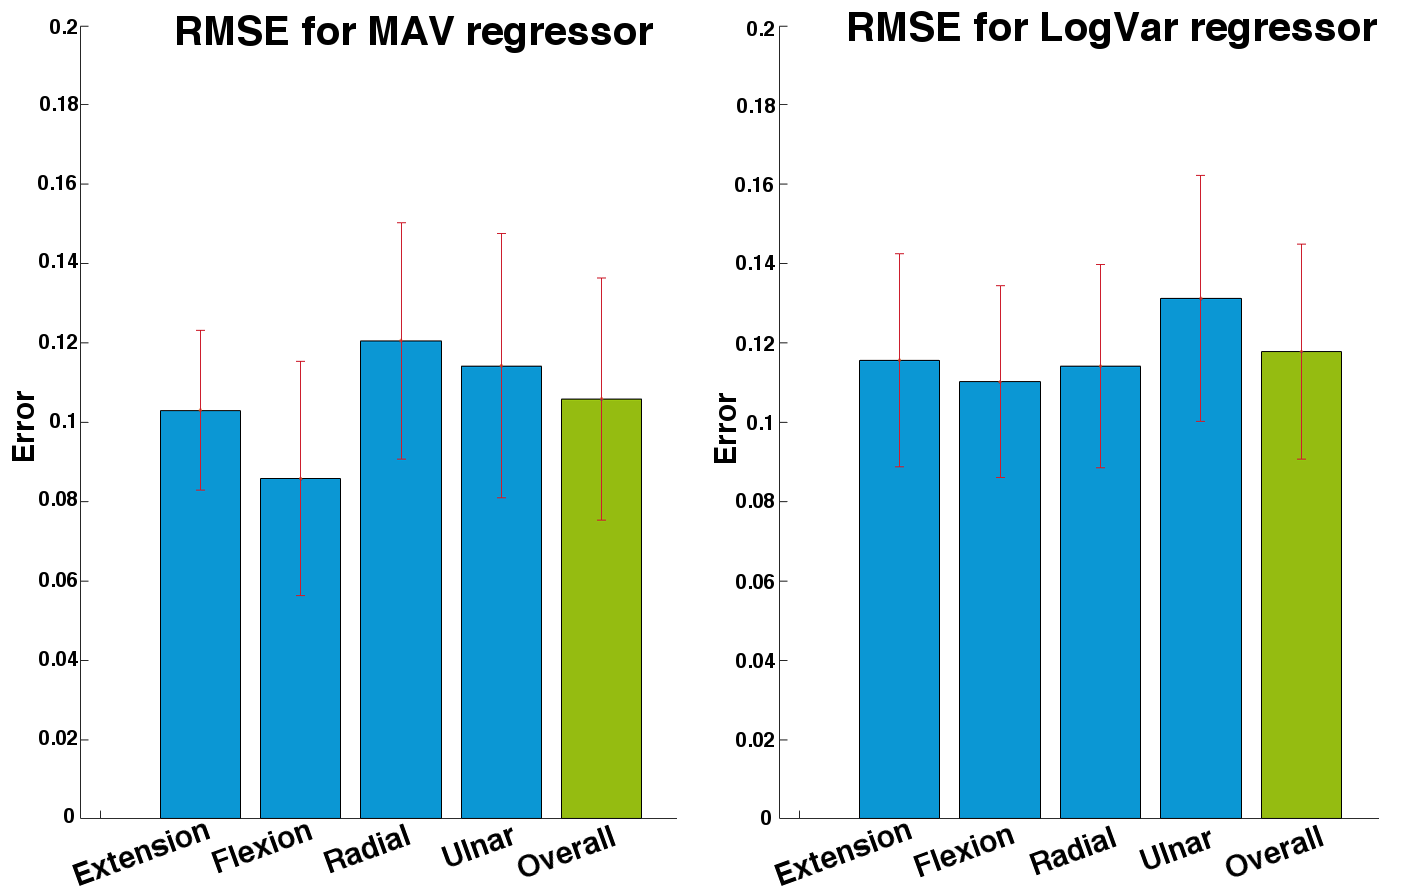
\includegraphics[width=1\textwidth]{figures/results/gimmeThemRMSEBars}  %<--but is not needed.
	\caption{Bar plot of the error of MAV and the LogVar features for the four hand gestures. The bar chart illustrates the mean error and the error bar illustrates the standard deviation}
	\label{fig:gimmeThemRMSEBars}  %<--give the figure a label, so you can reference!
\end{figure}

	\begin{center}
		\begin{tabular}{l l l}
			\toprule
			\textbf{Feature} & \textbf{Overall mean error} & \textbf{Standard deviation}\\
			\midrule
			Extension & 0.1030 & $\pm 0.0210$ \\
			Flexion & 0.1102 & $\pm 0.0296$ \\
			Radial Deviation & 0.1206 & $\pm 0.0298$ \\
			Ulnar Deviation & 0.1143 & $\pm 0.0334$ \\
			Overall & 0.1059 & $\pm 0.0306$ \\
			\bottomrule
		\end{tabular}
		\captionof{table}{RMSE for the implemented MAV regressor}
	\end{center}
	
	\begin{center}
		\begin{tabular}{l l l}
			\toprule
			\textbf{Feature} & \textbf{Overall mean error} & \textbf{Standard deviation}\\
			\midrule
			Extension & 0.1157 & $\pm 0.0469$ \\
			Flexion & 0.1102 & $\pm 0.0241$ \\
			Radial Deviation & 0.1142 & $\pm 0.0256$ \\
			Ulnar Deviation & 0.1312 & $\pm 0.0310$ \\
			Overall & 0.1178 & $\pm 0.0272$ \\
			\bottomrule
		\end{tabular}
		\captionof{table}{RMSE for the implemented LogVar regressor}
	\end{center}

The overall mean of the RMSE of MAV is 0.0943 with a standard deviation of $\pm 0.0290$, where the highest mean of a regressor is 0.1088 and the highest standard deviation is $\pm 0.0366$. The overall mean of the RMSE of LogVar is 0.1107 with a standard deviation of $\pm 0.0298$, where the highest mean of a regressor is 0.1216 and the highest standard deviation is $\pm 0.0402$. MAV then yields a lower mean RMSE and a lower standard deviation than LogVar - both with the overall RMSE and for the movement with the highest RMSE.


\textbf{Strahija says that we should consider including RMSE of the different intensities individually, to quantitatively express that both features(but especially LogVar) do poor control of higher intensities.}
%%% testing data plot
\subsection{Accuracy of regressors with test data}
This section contains the superimposition of the expected output of the regressors on the output of the regressors fed with test data. The plot in \figref{fig:SuperPoisonLogVarNewData} depicts the superimposition the logarithmic variace trained regressors fed with the test data.

\begin{figure}[H]
	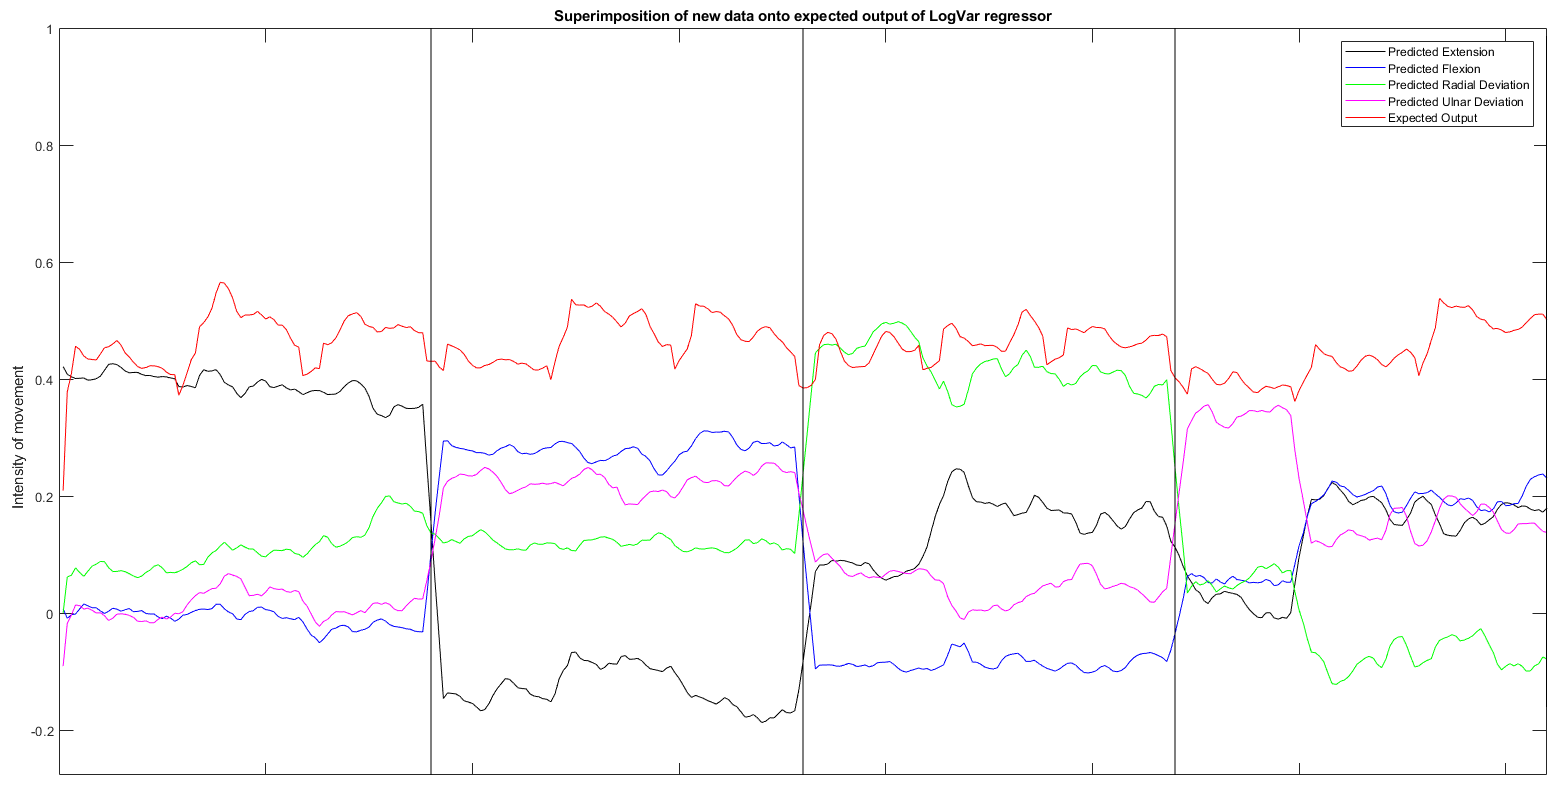
\includegraphics[width=1\textwidth]{figures/results/SuperPoisonLogVarNewData}  %<--but is not needed.
	\caption{}
	\label{fig:SuperPoisonLogVarNewData}  %<--give the figure a label, so you can reference!
\end{figure}

It is seen that regressors trained for different movements reacts on the same movement, especially for the flexion and ulnar deviation movement. However, the 

\begin{figure}[H]
	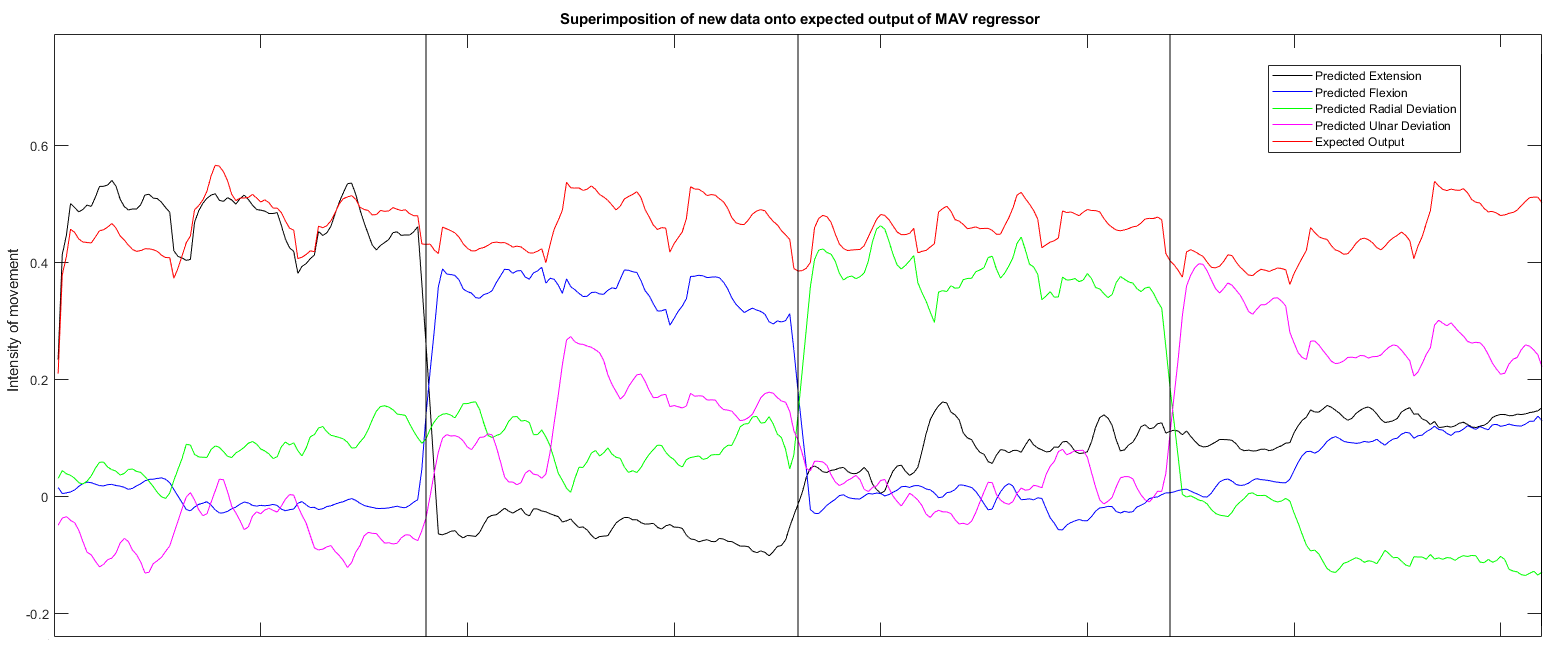
\includegraphics[width=1\textwidth]{figures/results/SuperPoisonMavNewData}  %<--but is not needed.
	\caption{}
	\label{fig:SuperPoisonMavNewData}  %<--give the figure a label, so you can reference!
\end{figure}


\begin{figure}[H]
	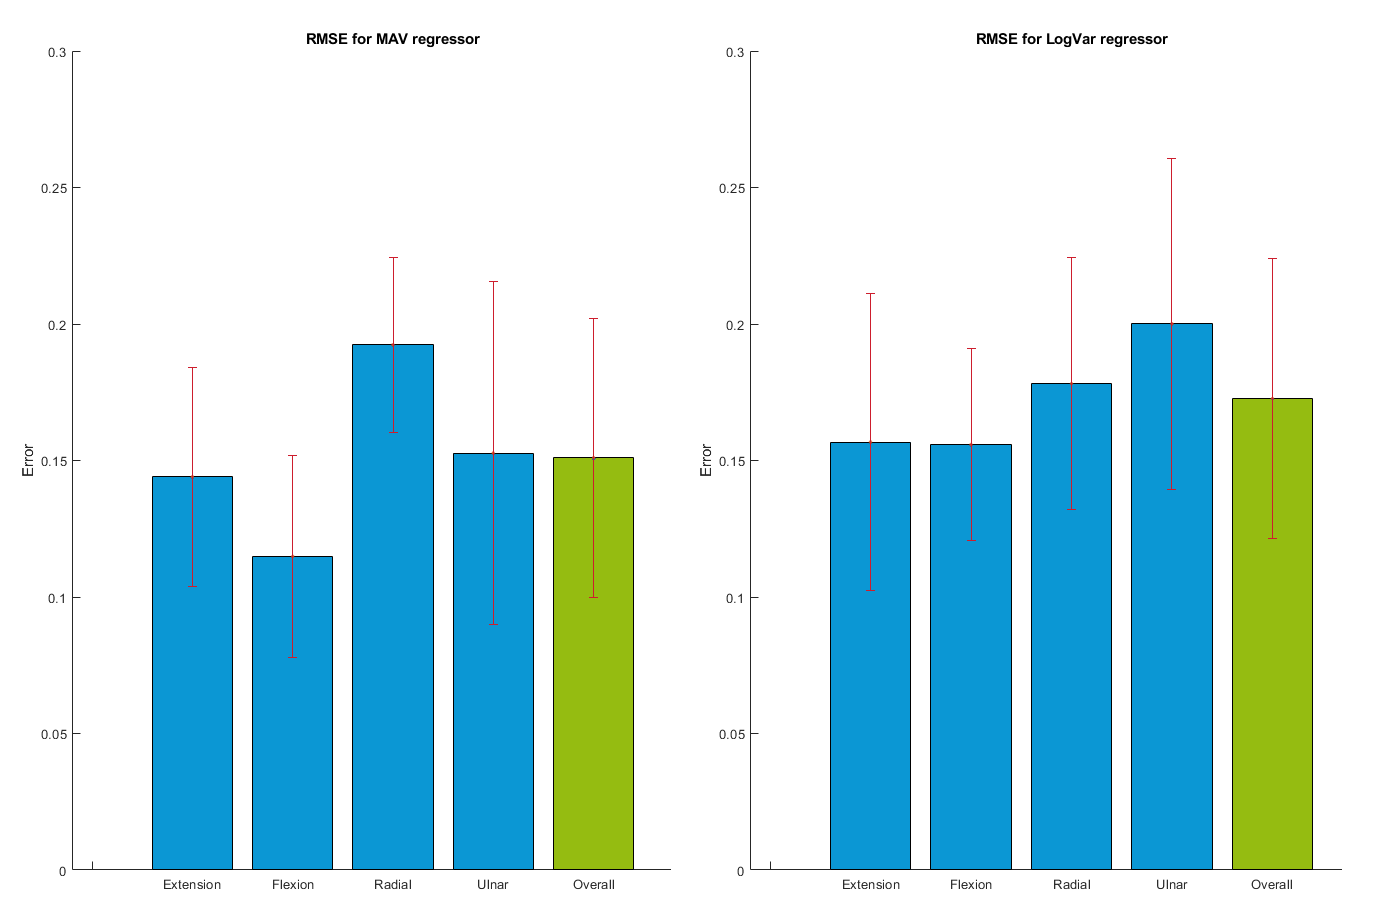
\includegraphics[width=1\textwidth]{figures/results/RMSEBarPlotNewData}  %<--but is not needed.
	\caption{}
	\label{fig:RMSEBarPlotNewData}  %<--give the figure a label, so you can reference!
\end{figure}

	\begin{center}
		\begin{tabular}{l l l}
			\toprule
			\textbf{Feature} & \textbf{Overall mean error} & \textbf{Standard deviation}\\
			\midrule
			Extension & 0.1646 & $\pm 0.0753$ \\
			Flexion & 0.1391 & $\pm 0.0841$ \\
			Radial Deviation & 0.2018 & $\pm 0.0424$ \\
			Ulnar Deviation & 0.1743 & $\pm 0.0905$ \\
			Overall & 0.1700 & $\pm 0.0759$ \\
			\bottomrule
		\end{tabular}
		\captionof{table}{RMSE for the implemented MAV regressor}
	\end{center}
	

	
	\begin{center}
		\begin{tabular}{l l l}
			\toprule
			\textbf{Feature} & \textbf{Overall mean error} & \textbf{Standard deviation}\\
			\midrule
			Extension & 0.1552 & $\pm 0.0514$ \\
			Flexion & 0.1680 & $\pm 0.0508$ \\
			Radial Deviation & 0.1681 & $\pm 0.0540$ \\
			Ulnar Deviation & 0.2078 & $\pm 0.0621$ \\
			Overall & 0.1748 & $\pm 0.0563$ \\
			\bottomrule
		\end{tabular}
		\captionof{table}{RMSE for the implemented LogVar regressor}
	\end{center}
	
		\begin{center}
			\begin{tabular}{l l}
				\toprule
				\textbf{Feature} & \textbf{P-Value}\\
				\midrule
				LogVar and MAV & 0.0044 \\
				LogVar new data and MAV new data & 0.1138 \\
				LogVar new data and LogVar & 0.0001 \\
				MAV new data and MAV & 0.000002 \\
				\bottomrule
			\end{tabular}
			\captionof{table}{P-Values for comparison of the features}
		\end{center}
		
It was found that the P-value of a Friedman's statistical test showed a significant difference (p = 0.0044) between the RMSE for the MAV and LogVar regressors with the training data as input, where LogVar has the higher mean. When examining the RMSE for the regressors with unknown test data consisting of 50\% contractions of all movements in all limb positions, it was shown that there is no significant difference (p = 0.1138) between the offline performance of the two regressors. When comparing the offline tests with training data and 50\% test data, it was shown that there's a significant difference for both LogVar (p = 0.000002) and LogVar (p = 0.0001), where the mean is higher for the unknown 50\% data in both cases.

\textbf{LOOK AT ME: We should do statistics to see if the RMSE of training differs from the test RMSE}